\section{Background}

\begin{frame}{Information Flow Basics}
	Information Flow considers \textit{confidentiality states}. Flow \textit{policies} formalise how information may move between states.
	
	Simple model: logical predicates.
	
	A more complex model: the Bell-LaPadula Lattice model (as used by the US military).
	
	\begin{figure}
		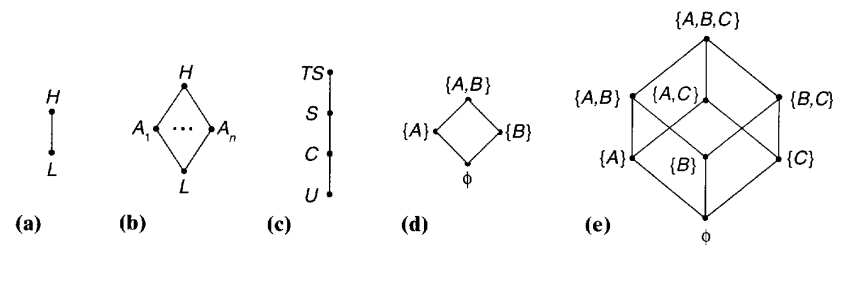
\includegraphics[scale=0.45]{content/images/lattice_examples.png}
		\caption{Example Lattice Model states \cite{ifbackground:sandhu}}
	\end{figure}
	
\end{frame}

\begin{frame}{Noninterference}
	
	A program which leaks no high confidentiality information is `noninterfering', but proving that a program is noninterfering is usually not practical.
	
%	\begin{block}{Noninterference}
%		A program is noninterfering if any two different executions which differ only in their high confidentiality inputs are indistinguishable to an attacker. \cite{ifbackground:goguen}
%	\end{block}
	
	\begin{itemize}
		\item Proving noninterference (in the general case) is undecidable
			\begin{itemize}
				\item The halting problem can be reduced to it
			\end{itemize}
		\item Many useful programs are inherently interfering
			\begin{itemize}
				\item A password checker's output clearly depends on the password
			\end{itemize}
	\end{itemize}
	
	Most real systems allow for \textit{selective declassification}.
\end{frame}

%\begin{frame}{Noninterference - Is It Practical?}
%	Problems with proving noninterference:
%	
%	\begin{enumerate}
%		\item Proving non-interference (in the general case) is undecidable
%			\begin{itemize}
%				\item The halting problem can be reduced to it -- consider: \newline \texttt{\textbf{if} S() halts \textbf{then} h := 1 \textbf{else} h := 0} \cite{ifbackground:denninghalting}
%				\item \textit{Most real systems prove a simplified case using type checking}
%			\end{itemize}
%		\item Many useful programs are inherently interfering
%			\begin{itemize}
%				\item A password checker's output clearly depends on the password
%				\item \textit{Most real systems allow for `selective declassification'}
%			\end{itemize}
%		\item Noninterference does not model covert channels
%			\begin{itemize}
%				\item \textit{Some systems secure against specific potential covert channels}
%				\item There is no way to prove that no covert channels exist
%			\end{itemize}
%	\end{enumerate}
%\end{frame}

\begin{frame}{Enforcement: Static or Dynamic?}
	Flow controls be enforced at compile-time or at run-time.
	
	\textbf{Dynamic} information flow controls:
	\begin{itemize}
		\item Flexible: can represent policies which change dynamically
		\item Incur some run-time overhead
		\item Can only track the code path which is executed
	\end{itemize}
	
	\textbf{Static} information flow controls:.
	\begin{itemize}
		\item Have little or no run-time overhead
		\item Can easily track \textit{all} possible code paths
	\end{itemize}
	
	Most solutions use static or `mostly static' approaches.
\end{frame}

%\begin{frame}{Information Flow and Integrity}
%	Information flow is usually talked about with respect to confidentiality, but it can also be applied to integrity.
%	
%	For \textbf{Confidentiality}:\newline Track the flow of high confidentiality (`secret') outputs.
%	
%	For \textbf{Integrity}:\newline Track the flow of low integrity (`tainted') inputs.
%\end{frame}